%!TEX program = xelatex
\documentclass{beamer}

\usepackage{blindtext}

\usepackage{fontenc} % added by Aurelie Jean 

\usetheme{Execushares}

\definecolor{isvblue}{RGB}{37,5,247} % ISV blue color (#2505F7)

\linespread{1.5}

\title{Digitalo-Analytic Transformation:\\The Power of Data \\Which role can we play? What are our strength? How to be better prepared?}
\subtitle{\textcolor{isvblue}{\textit{Coding for a brighter and better future for everyone}}}

\titlegraphic{
\includegraphics[width=0.30\textwidth]{./pictures/chanel.jpg}\hspace{5.0cm}
              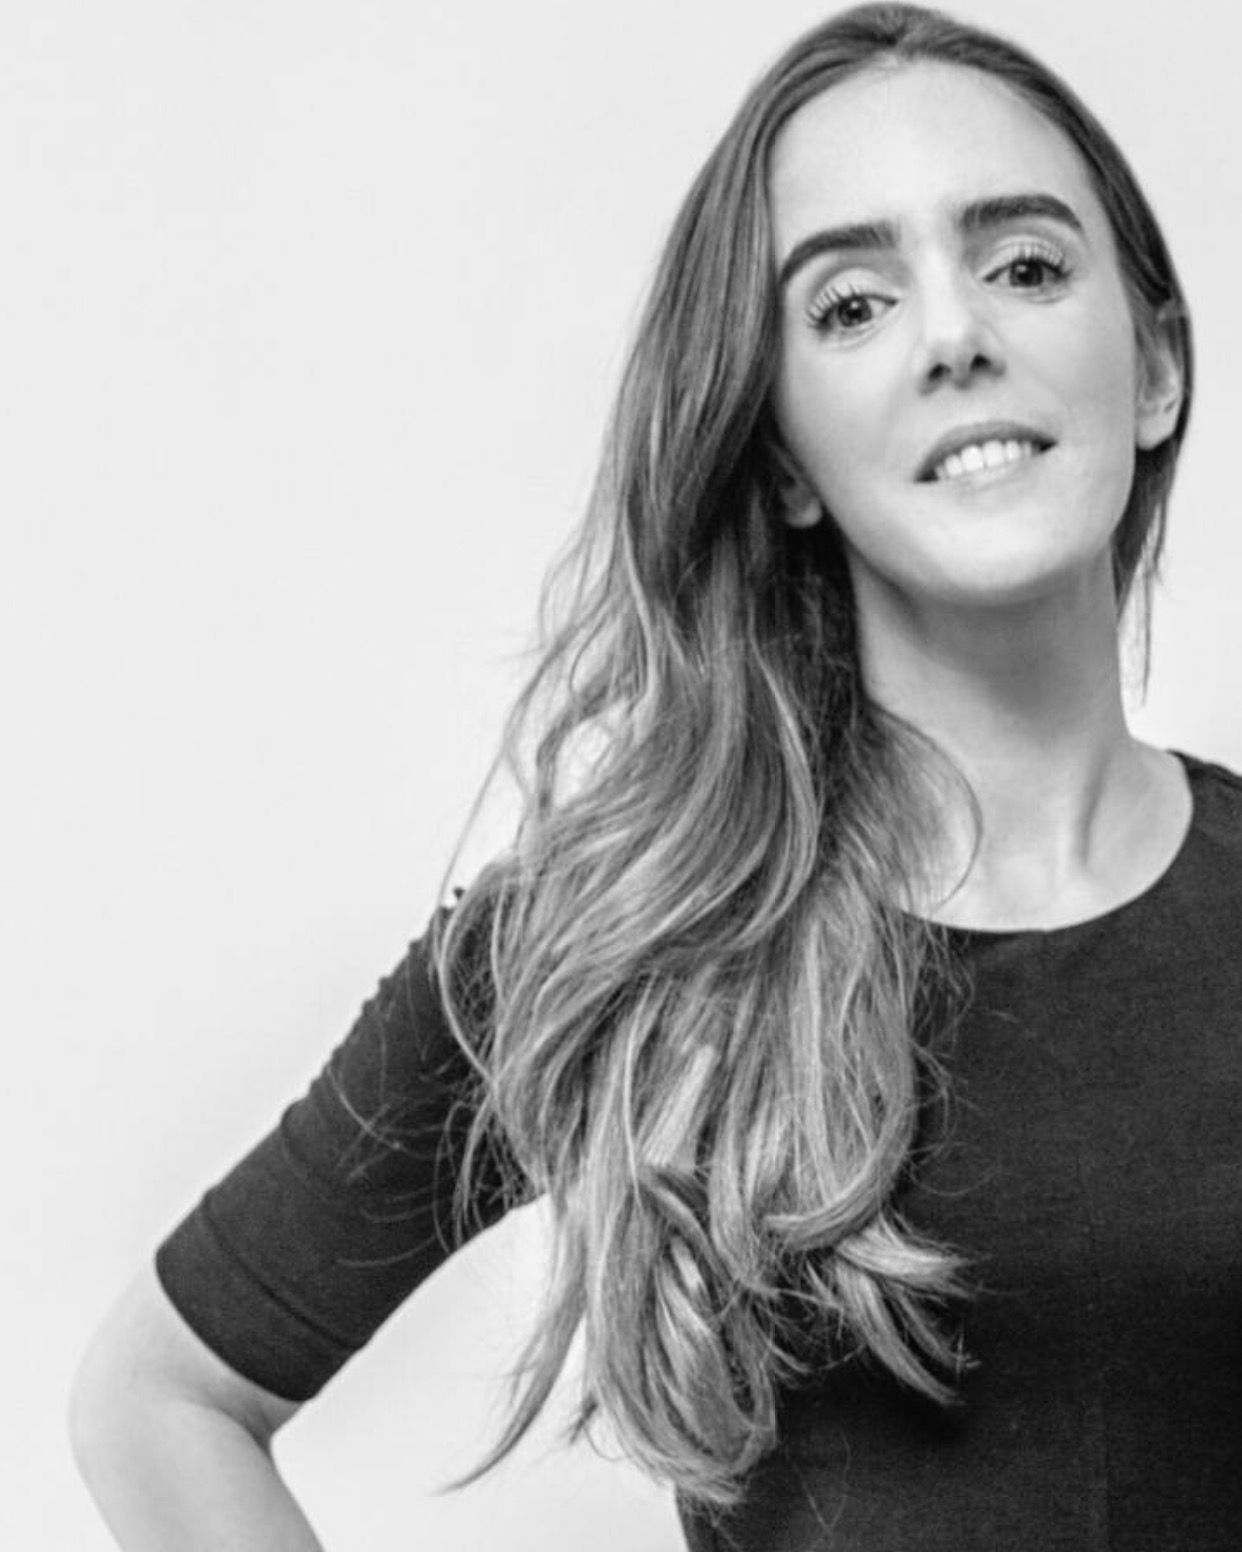
\includegraphics[width=0.26\textwidth]{./pictures/Aurelie-Jean_2016_001.JPG}}

\author{Dr. Aur\'elie JEAN, PhD}
\institute{\textcolor{isvblue}{In Silico Veritas, LLC} - aurelie@silicoveritas.com}
\date{seminar Chanel NYC - May, 24th 2017}

%\setcounter{showSlideNumbers}{1}

\begin{document}
	\setcounter{showProgressBar}{0}
	\setcounter{showSlideNumbers}{0}

        \begin{frame}%[label=pageone]
        \maketitle
        \end{frame}


	\setcounter{framenumber}{0}
	\setcounter{showProgressBar}{1}
	\setcounter{showSlideNumbers}{1}

        
% PART 0
        \section{Microprocessor Technology Revolution}
        \begin{frame}
\frametitle{3rd industrial (numerical) revolution}
\vskip 1.1cm
\begin{center}
    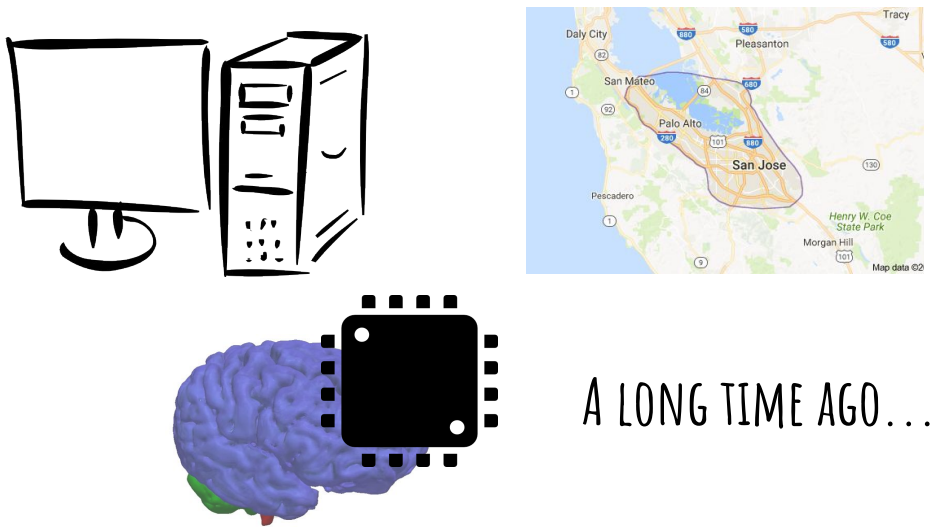
\includegraphics[width=0.9\textwidth]{./pictures/computer-microprocessor.png}
\end{center}
%\vspace{-0.5cm}
\vskip 0.3cm
%\hspace{9.0cm}
\tiny{Source: personal, FreeDownload, Google Map}

\end{frame}



        \section{What has changed today?}
        \begin{frame}
\frametitle{Our relationship with Technology}
\vskip 1.15cm
\begin{center}
    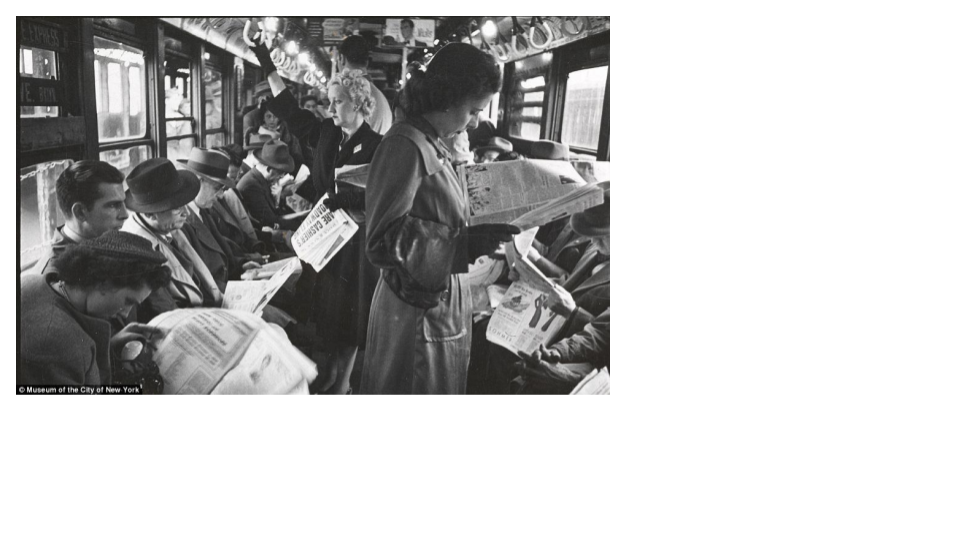
\includegraphics[width=1.0\textwidth]{./pictures/OldTime.png}
\end{center}
%\vspace{-0.5cm}
\tiny{Source: S. Kubrick for Look magazine / Museum of City of NY. X2011.4.10292.30D ©SK Film Archives, D. Guttenfelder/National Geographic Creative}
\end{frame}

\begin{frame}
\frametitle{Our relationship with Technology}
\vskip 1.08cm
\begin{center}
    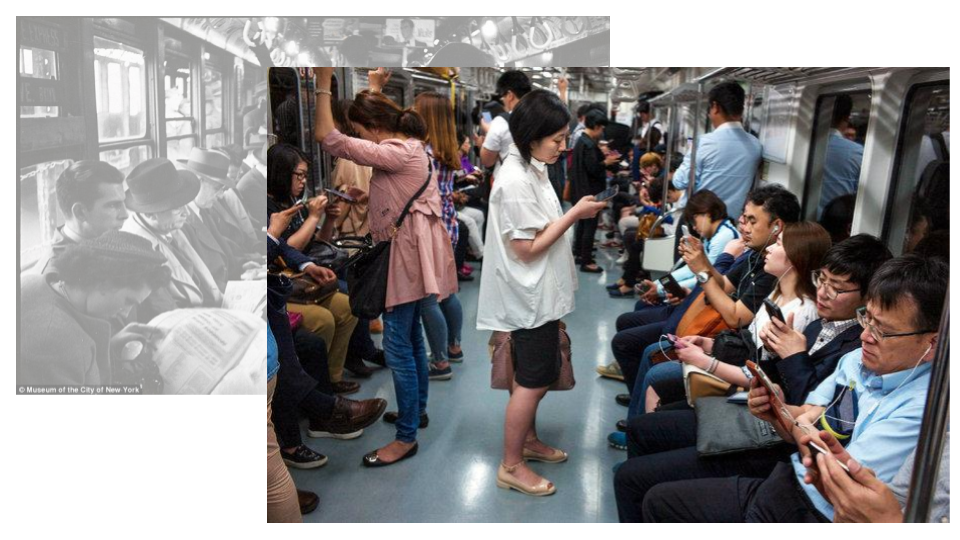
\includegraphics[width=1.0\textwidth]{./pictures/NewTime.png}
\end{center}
%\vspace{-0.5cm}
\tiny{Source: S. Kubrick for Look magazine / Museum of City of NY. X2011.4.10292.30D ©SK Film Archives, D. Guttenfelder/National Geographic Creative}
\end{frame}



        \section{To touch people, you have to talk to their connected device}


% PART 1
        \section{Digitalo-Analytic Transformation}
        \begin{frame}
\frametitle{Digital Transformation}
\vskip 1.1cm

\includegraphics[width=1.0\textwidth]{./pictures/reachClients.png}
\end{frame}


        \begin{frame}
\frametitle{Digitalo-Analytic Transformation}
\vskip 1.0cm
\vspace{0.5cm}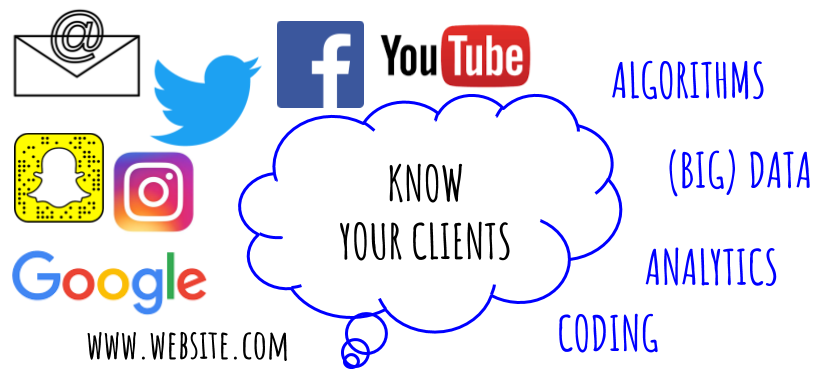
\includegraphics[width=1.00\textwidth]{./pictures/knowClients.png}
\end{frame}


        \section{Diversity will drive the success of this transformation!}
        \begin{frame}
\frametitle{Diversity: a large definition }
\vskip 0.7cm
\hspace{-1.0cm}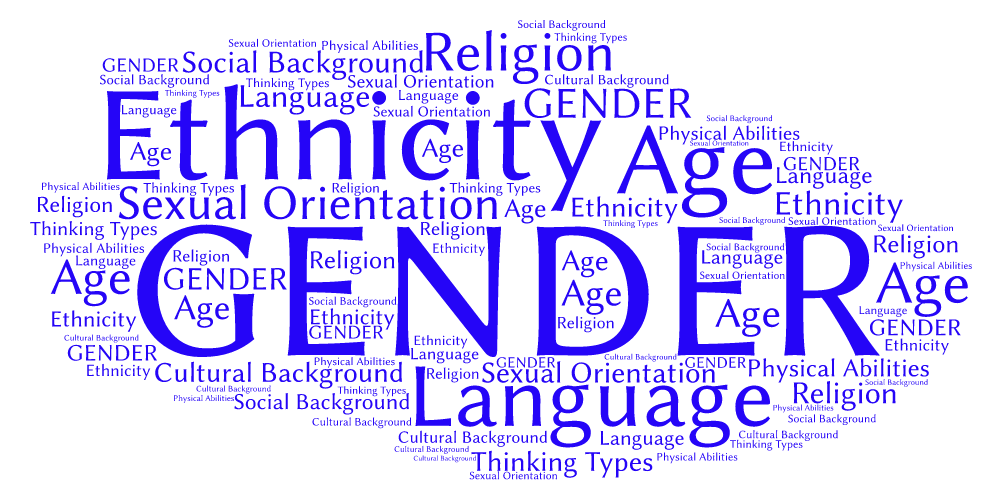
\includegraphics[width=1.1\textwidth]{./pictures/Word-Cloud-diversity.png}
\vskip 0.3cm
\emph{``The art of thinking independently together"} M. Forbes.
    %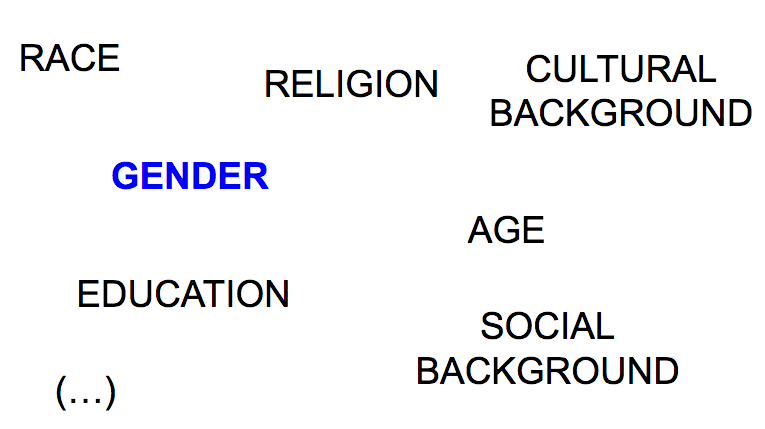
\includegraphics[width=1.0\textwidth]{./pictures/diversity-definition.png}
\end{frame}


        \begin{frame}
\frametitle{Positive Impacts of Diversity}
\vskip 0.7cm
\textcolor{isvblue}{DIVERSITY IS GOOD FOR BUSINESS!}
\begin{itemize}
\item increases \textcolor{isvblue}{adaptability} and \textcolor{isvblue}{flexibility}
\item enlarges \textcolor{isvblue}{viewpoints} and, enriches \textcolor{isvblue}{new} and \textcolor{isvblue}{novel ideas}
\item encourages employees to \textcolor{isvblue}{outperform}
\item attracts more \textcolor{isvblue}{talented people}
\item (...)
\end{itemize}

\vskip 0.2cm
$\rightarrow$ awareness of investors, companies, governments:  BFGEI Bloomberg Financial Gender-Equality Index

\vskip 0.4cm
\tiny{(Jha, 2009)(Saxena, 2014)(McKinsey, 2015)(Sandberg, 2016)(Parker, 2016)...}
\end{frame}

\begin{frame}
\frametitle{Diversity is good for this Transformation}
\vskip 0.7cm
\textcolor{isvblue}{DIVERSITY IS A POSITIVE DISRUPTER THAT SUPPORTS TRANSFORMATION!}
\begin{itemize}
\item \textcolor{isvblue}{Diversity helps transform faster}: more people with different visions who adapt faster to continuously evolving environment
\item \textcolor{isvblue}{Diversity helps transform better and deeper}: employees with a high adaptibility accept, encourage and proactively engage in this transformation
\item (...)
\end{itemize}
\end{frame}

\begin{frame}
\frametitle{Benefits of this transformation for Women}
\vskip 0.4cm
\begin{itemize}
\item \textcolor{isvblue}{Larger job market with competitive salaries} and possibility to work in any field 
\item Opportunity to \textcolor{isvblue}{create next generation tools} to \textcolor{isvblue}{impact our society} 
\item An \textcolor{isvblue}{entire ecosystem to create}: everything needs to be learned, transformed and adapted
\item \textcolor{isvblue}{New workplace's rules and metrics of success} to build
\item \textcolor{isvblue}{Re-organization of the structure of companies} that helps women grow faster, more transverse management
\end{itemize}

\end{frame}


% PART 2
	\section{(Big) Data: a technological and human transformation}
        \begin{frame}
\frametitle{What is (Big) Data?}
\vskip 1.0cm
\textit{From Wikipedia: \textcolor{isvblue}{qualitative or quantitative} variables for analysis}
    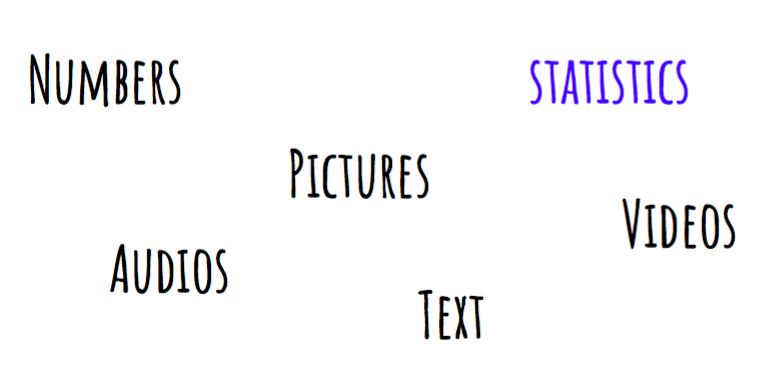
\includegraphics[width=1.0\textwidth]{./pictures/data-what.png}\\
\textcolor{isvblue}{The size of the data is a \textbf{spatiotemporal notion}!} 
\end{frame}

\begin{frame}
\frametitle{What do we do with (Big) Data?}
\vskip 0.8cm
Analyze (Big) Data to \textcolor{isvblue}{understand} and make some \textcolor{isvblue}{predictions} in:
\begin{itemize}
  \item \textcolor{isvblue}{Medicine}: to accelerate diagnosis and personnalize treatments  
  \item \textcolor{isvblue}{Government authorities}: to improve infrastructures and city operations (ex: Open Data platform by NYC)
  \item \textcolor{isvblue}{Social research}: to deepen understand social demography
  \item \textcolor{isvblue}{Marketing}: to understand customers and target strategies
  \item \textcolor{isvblue}{Journalism}: to investigate (Matt Caroll from Spotlight)
  \item (...) \textcolor{isvblue}{To innovate}
\end{itemize}
\end{frame}

\begin{frame}
\frametitle{Progress, Challenges, which Role to play?}
\vskip 0.8cm
    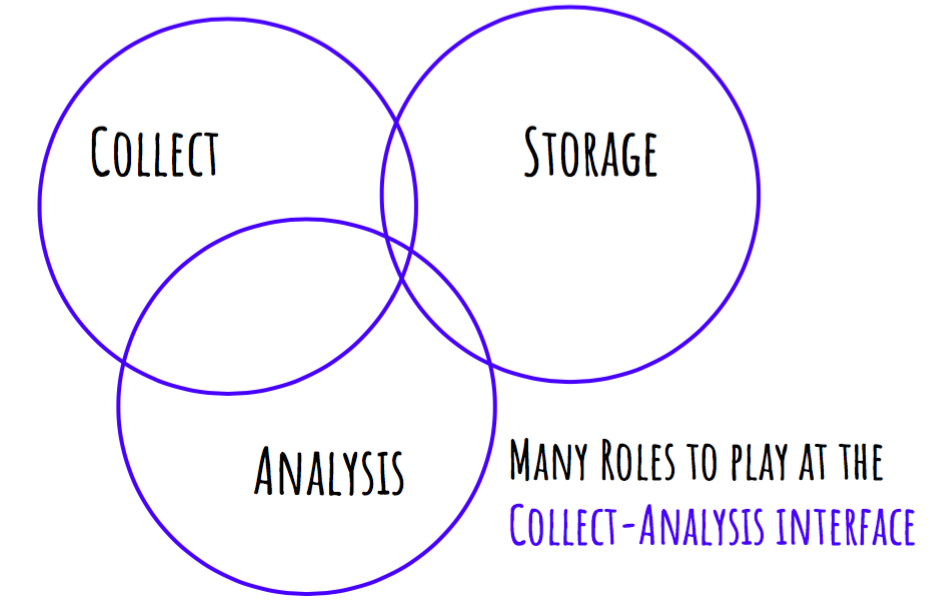
\includegraphics[width=1.0\textwidth]{./pictures/roles-in-data.png}\\
\end{frame}

\begin{frame}
\frametitle{(Big) Data Collect-Analysis interface}
\vskip 1.0cm
    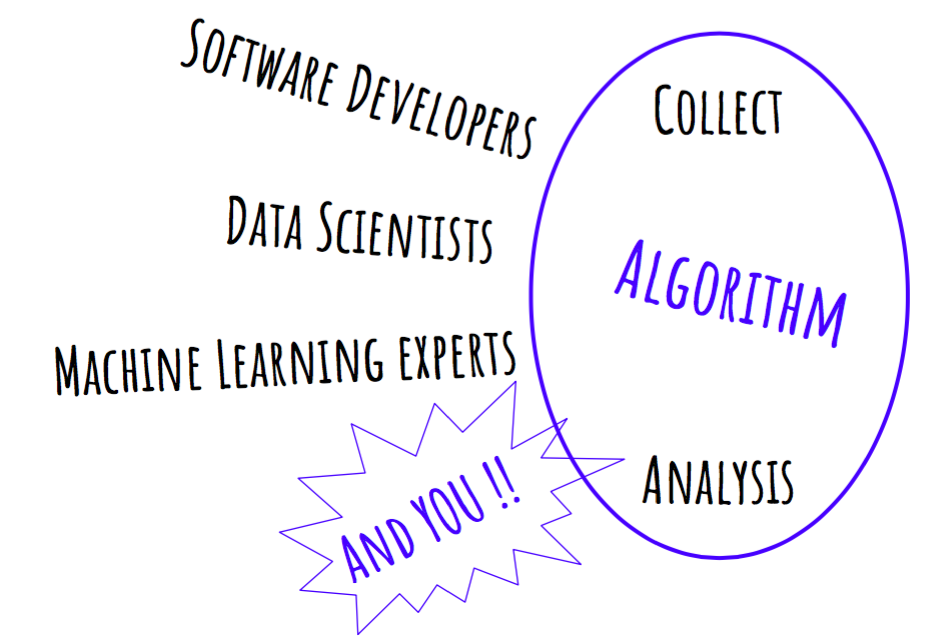
\includegraphics[width=1.0\textwidth]{./pictures/role-2.png}\\

\end{frame}



% PART 3
       \section{Coding is the best valuable asset to embrace this transformation}
        \begin{frame}
\frametitle{Why learn how to Code?}
\vskip 0.8cm
\begin{itemize}
    \item \textcolor{isvblue}{Communicate efficiently} with tech teams
    \item \textcolor{isvblue}{Closely collaborate} with developers and scientists
    \item \textcolor{isvblue}{Give insightful input} to better collect and analyze data
    \item \textcolor{isvblue}{Understand} underlying mechanisms of new technologies
    \item \textcolor{isvblue}{Innovate and transform} faster and better
    \item \textcolor{isvblue}{Become a next-generation leader!}
\end{itemize}
\end{frame}




\end{document}
